%**8-page Report Framework**
%
%1. Abstract (emphasize our variants)
%2. Introduction & Related Works (1 page)
%3. Formulation (1 page)
%4. Feature Extraction (2 pages)
%5. Learning (0.5 page)
%6. CRF Inference (0.5 page)
%7. Pixel Level result presentation (1 page)
%8. Result evaluation in rectangle level (1 page)
%9. Discussion (existing flaws and possible improvements) (0.5 page)
%10. acknowlegement and reference (0.5 page)
%
\documentclass[10pt,twocolumn,letterpaper]{article}

\usepackage{iccv}
\usepackage{times}
\usepackage{epsfig}
\usepackage{graphicx}
\usepackage{amsmath}
\usepackage{amssymb}

\DeclareMathOperator*{\argmin}{arg\,min}
\DeclareMathOperator*{\argmax}{arg\,max}
\newcommand{\SUM}{\sum\limits}
\newcommand{\hs}{\hspace{0.58in}}
\newcommand{\BOLD}{\textbf}
% Include other packages here, before hyperref.

% If you comment hyperref and then uncomment it, you should delete
% egpaper.aux before re-running latex.  (Or just hit 'q' on the first latex
% run, let it finish, and you should be clear).
\usepackage[pagebackref=true,breaklinks=true,letterpaper=true,colorlinks,bookmarks=false]{hyperref}

\iccvfinalcopy % *** Uncomment this line for the final submission
\def\iccvPaperID{****} % *** Enter the ICCV Paper ID here
\def\httilde{\mbox{\tt\raisebox{-.5ex}{\symbol{126}}}}

% Pages are numbered in submission mode, and unnumbered in camera-ready
\ificcvfinal\pagestyle{empty}\fi
\begin{document}

%%%%%%%%% TITLE
\title{Application of Conditional Random Fields to Pixel-Level Salient Object Detection Through Local, Regional and Global Features}
%\title{Application of Conditional Random Field in Image Salient Object Detection\\ with Local, Regional and Global Feature Extraction}

\author{Jimmy Lin\\
Australian National University\\
Canberra, Australia\\
{\tt\small \url{linxin@gmail.com}}
% For a paper whose authors are all at the same institution,
% omit the following lines up until the closing ``}''.
% Additional authors and addresses can be added with ``\and'',
% just like the second author.
% To save space, use either the email address or home page, not both
\and
Christopher Claou\'e-Long\\
Australian National University\\
Canberra, Australia\\
{\small\url{u5183532@anu.edu.au}}
}

\maketitle
% \thispagestyle{empty}

%%%%%%%%% ABSTRACT
\begin{abstract}
Making use of OpenCV, DARWIN and the MSRA dataset, we detect the saliency of an object in an image by extracting local, regional and global saliency features at the pixel level, then combine those features with pre-fitted weights derived by logistic regression. A conditional random field is then constructed to capture the spatial continuity of the salient object, with a weighting ratio of combined unary and pairwise terms that is determined by cross-validation \BOLD{LOGISTIC REGRESSION?}. The binary mask inferred by the conditional random field is then used to output a single bounding rectangle around a salient area through a winner-takes-all algorithm to label the detected salient object, by which the performance of our approach is evaluated through mean boundary displacement error. 
\end{abstract}

%% Introduction & Related Works (1 page)
\section{Introduction and Motivation}

A long-standing problem in the field of computer vision is how to calculate the saliency of objects in an image, that is, their prominence in the image when compared to their background and surrounds.  Human vision can accomplish this quite easily, since the human brain has mechanisms to direct attention to the main objects in the perceived image.  This visual attention has been studied by researchers in multiple fields, from physiology and psychology to computer vision.  The property of detecting a salient object is important for the latter because it leads to the ability to single out individual areas of an image, for example in automatic image cropping and vision simulation in robotics, as well as 3D surface reconstruction in augmented reality displays.

\begin{figure}[h]
\begin{center}
    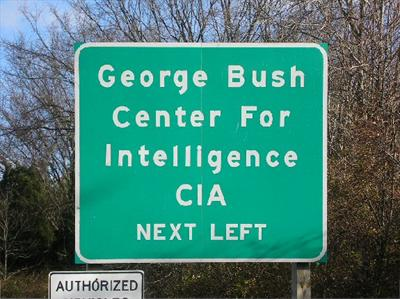
\includegraphics[width=0.6in,height=0.4in]{./Figures/example_image/4_140_140907.jpg}
    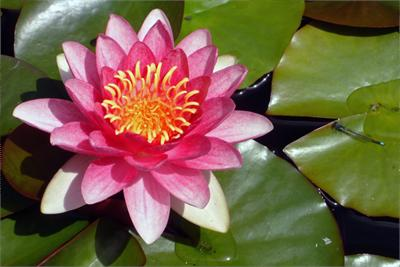
\includegraphics[width=0.6in,height=0.4in]{./Figures/example_image/4_141_141474.jpg}
    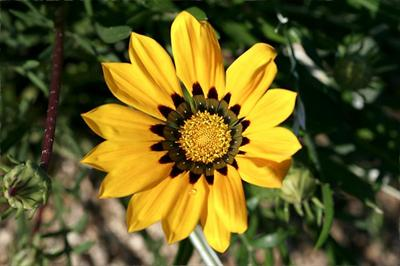
\includegraphics[width=0.6in,height=0.4in]{./Figures/example_image/4_141_141906.jpg}
    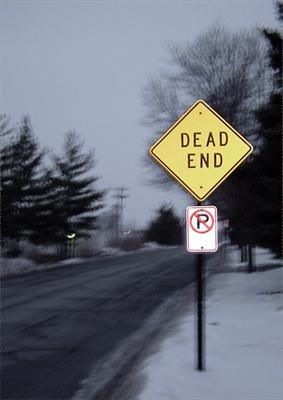
\includegraphics[width=0.6in,height=0.4in]{./Figures/example_image/4_142_142237.jpg}
    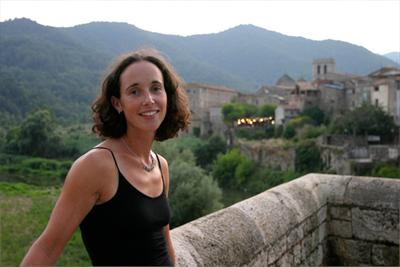
\includegraphics[width=0.6in,height=0.4in]{./Figures/example_image/4_142_142635.jpg}\\
    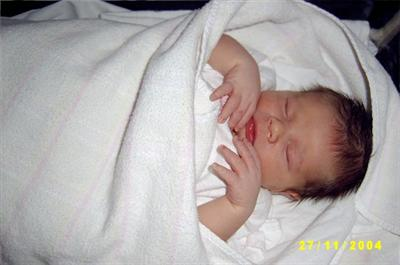
\includegraphics[width=0.6in,height=0.4in]{./Figures/example_image/4_124_124377.jpg}
    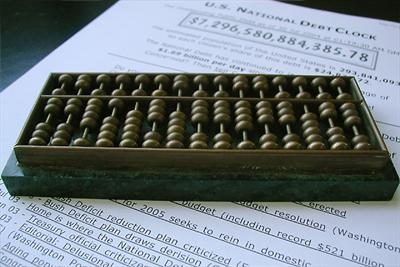
\includegraphics[width=0.6in,height=0.4in]{./Figures/example_image/4_124_124385.jpg}
    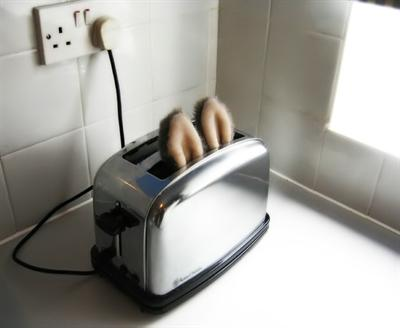
\includegraphics[width=0.6in,height=0.4in]{./Figures/example_image/4_124_124475.jpg}
    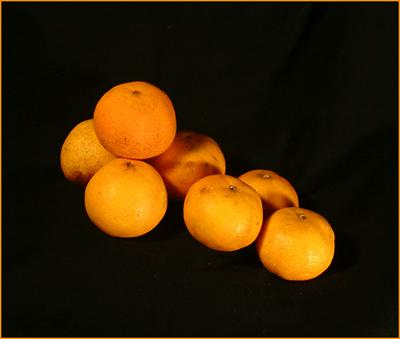
\includegraphics[width=0.6in,height=0.4in]{./Figures/example_image/4_124_124483.jpg}
    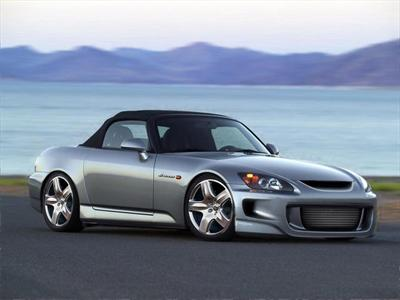
\includegraphics[width=0.6in,height=0.4in]{./Figures/example_image/4_128_128511.jpg} \\
    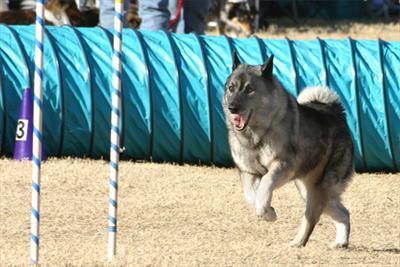
\includegraphics[width=0.6in,height=0.4in]{./Figures/example_image/4_129_129409.jpg}
    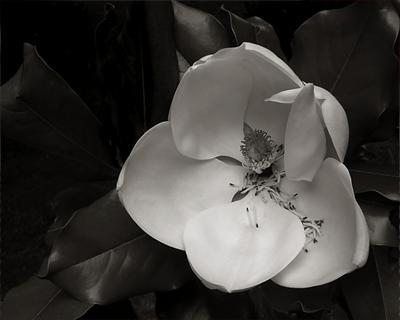
\includegraphics[width=0.6in,height=0.4in]{./Figures/example_image/4_132_132238.jpg}
    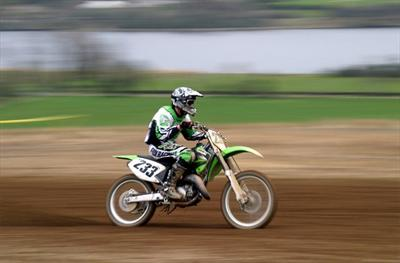
\includegraphics[width=0.6in,height=0.4in]{./Figures/example_image/4_135_135774.jpg}
    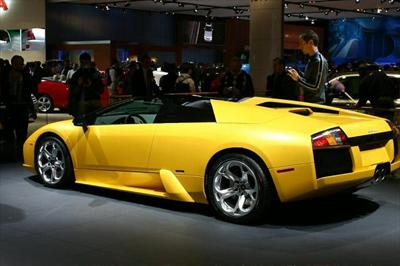
\includegraphics[width=0.6in,height=0.4in]{./Figures/example_image/4_136_136057.jpg}
    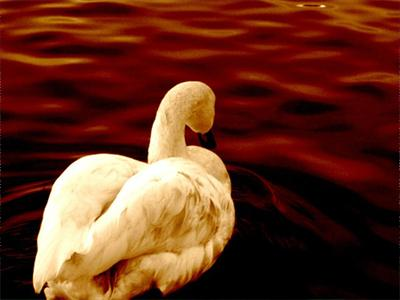
\includegraphics[width=0.6in,height=0.4in]{./Figures/example_image/4_136_136687.jpg}\\
    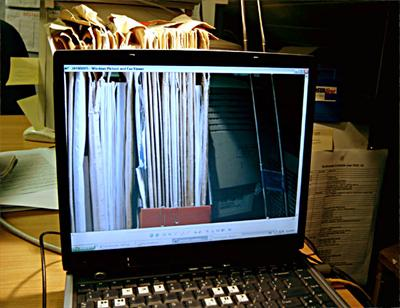
\includegraphics[width=0.6in,height=0.4in]{./Figures/example_image/4_137_137444.jpg}
    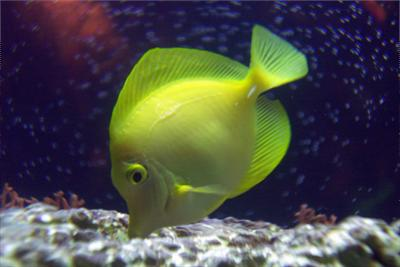
\includegraphics[width=0.6in,height=0.4in]{./Figures/example_image/4_138_138371.jpg}
    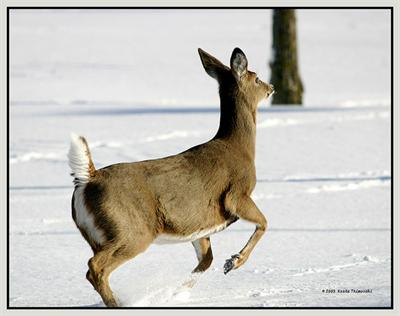
\includegraphics[width=0.6in,height=0.4in]{./Figures/example_image/4_139_139245.jpg}
    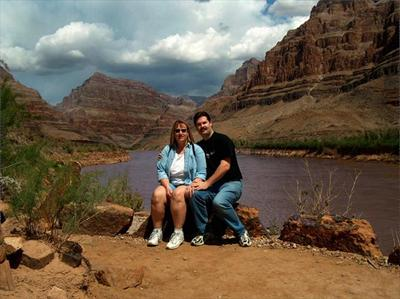
\includegraphics[width=0.6in,height=0.4in]{./Figures/example_image/4_139_139680.jpg}
    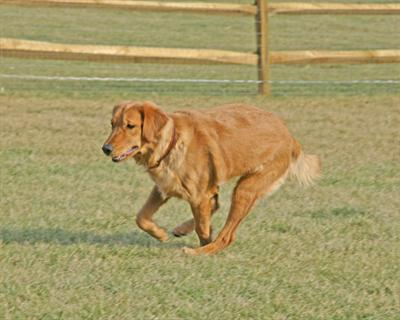
\includegraphics[width=0.6in,height=0.4in]{./Figures/example_image/4_140_140285.jpg}\\
    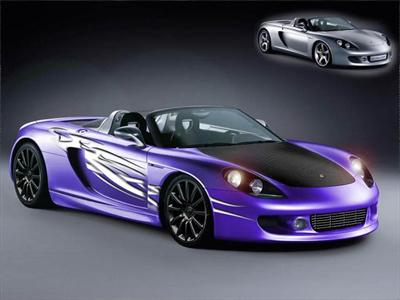
\includegraphics[width=0.6in,height=0.4in]{./Figures/example_image/4_142_142916.jpg}
    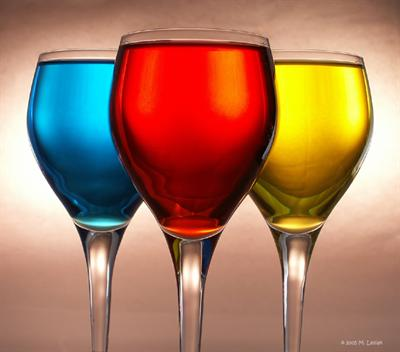
\includegraphics[width=0.6in,height=0.4in]{./Figures/example_image/4_143_143262.jpg}
    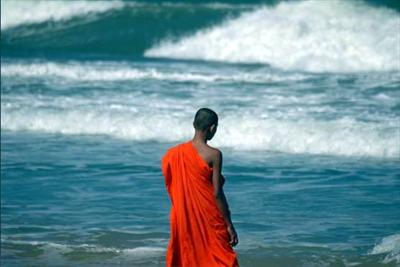
\includegraphics[width=0.6in,height=0.4in]{./Figures/example_image/4_144_144604.jpg}
    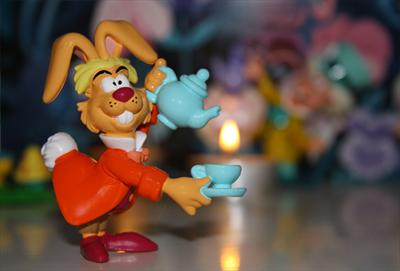
\includegraphics[width=0.6in,height=0.4in]{./Figures/example_image/4_134_134777.jpg}
    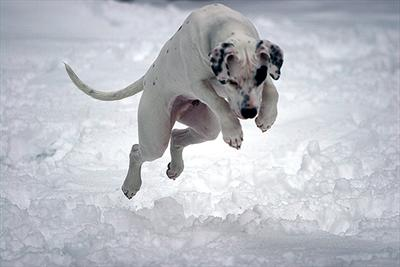
\includegraphics[width=0.6in,height=0.4in]{./Figures/example_image/4_134_134664.jpg}\\
    \caption{Example images from MSRA dataset B}
    \end{center}
\end{figure}

%% Related Works (0.5 page)
\section{Related Works}
Most existing approaches are based on a bottom-up computational framework, where the computer's simulation of visual attention is driven by low-level stimuli in the scene.  % as color intensity and contrast. 
These approaches employ three steps.

The first step is feature extraction, where multiple low-level visual features such as intensity, colour, orientation, texture, and motion are extracted from the image at multiple scales.

The second step is saliency computation. The saliency is computed by a centre-surround operation, self-information, or graph-based random walk using multiple features. After normalisation and linear/nonlinear combination, a master or saliency map is computed to represent the saliency of each pixel in the image. 

The last step is label output, where a few key locations on the saliency map are identified by winner-take-all, or inhibition-of- return, or other nonlinear operations.

%% Formulation (1 page)
\section{Our Approach}
In our approach, we base our salient object detection on several suppositions that mimic how human vision differentiates salient objects from the rest of the perceived field of view.  As can be observed in \BOLD{REDO FIGURES}, people naturally pay more attention to salient objects in images, such as a person, a face, a car, an animal, or a road sign. This is because of several reasons.

First of all, it is likely that pixels with a high contrast difference to their near neighbours to be part of a salient object, since they could represent a contour or boundary around an object.  This is similar to how the human brain discovers boundaries between objects in its visual field by detecting differences in light intensity\BOLD{CITATION PSYCHBOOK}.

Salient objects are more often than not quite distinct from their local surrounding region.  Calculating the distance between an object and its surrounds can therefore give us information about how salient that object is.  If we apply this concept over the entire image, we can gather information about how different various areas are to their surrounds and work out the likelihood that parts of an image are salient.

Finally, humans perceive prominence in objects through how distinct they are from their surrounds.  Indeed, salient objects often demonstrate a marked difference in colour to the rest of a scene.  Therefore, the more widely distributed a colour is in an image, the less likely it is that the salient object will contain that colour.  This global colour distribution can therefore be used to describe the saliency of the pixels in an image.

\subsection{Formulation}

To turn the problem of salient object detection into a mathematical formulation, we incorporate these three high-level concepts of a salient object into the process of creating a saliency map.  Salient object detection can be formulated this way as a binary labelling task that separates a salient object from the background through multiple operations.

For each pixel $x$ of given an image $I$, the binary mask $A_x$ must indicate whether it belongs to the salient object (1) or not (0). Our objective is to compute this mask $A$ in order to show the location of the salient object in the image.

To do this, we build up a probabilistic model $$P(A|I)=\frac{1}{Z}e^{-E(A|I)}$$ to determine the probability of a binary mask over an image with $\frac{1}{Z}$ as the normalising factor, and $E(A|I)$ as an energy function incorporating both unary and pairwise potentials between pixels in the image

\begin{figure}[h]
    \begin{center}
        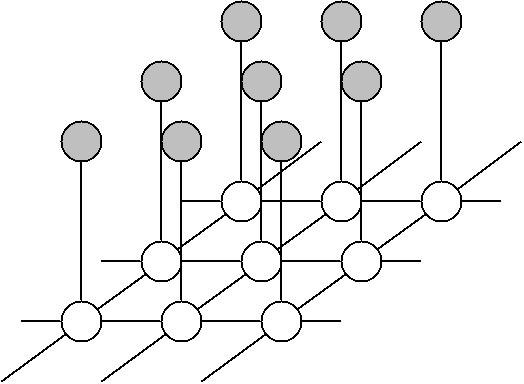
\includegraphics[width=1.8in,height=1in]{./Figures/mrf.jpg} \\
        \caption{A Conditional Random Field }\small White nodes are the objects, grey nodes are their potentials
        \end{center}
\end{figure}

Formally, the energy function can be represented as $$E(A|I) = \SUM_x S_{unary}(a_x,I) + \lambda_0 \SUM_{x,x'}S_{pair}(a_x,a_{x'},I)$$ where $\lambda$ is the relative weight between the sum of multiple unary  and pairwise features. 

The unary potential, combining the three pixel features, is specified as $$S_{unary}(a_x,I) = \SUM_{k=1}^K \lambda_k \cdot F_k(a_x,I)$$ where $\lambda_k$ is the cross-validated \BOLD{LOGISTIC REGRESSION?} weight of the $k^{th}$ feature such that $\sum_{k=1}^{K} \lambda_k = 1$.

The pairwise feature $S(a_x,a_{x'},I)$ exploits the spatial relationship between two adjacent pixels.  It can be viewed as a ``penalty'' for labelling adjacent pixels differently: $$S(a_x,a_{x'},I) = |a_x-a_{x'}| \cdot e^{-\beta d_{x,x'}}$$ where $x,x'$ represent two adjacent pixels, $d_{x,x'}$ is the L2-norm (standard norm) representing the colour difference between the two pixels, and $\beta=(2\langle||I_x-I_{x'}||^2\rangle)^{-1}$ is a robust parameter to weight the colour contrast.

\begin{figure}[h]
    \begin{center} %% image 5_156_156422
    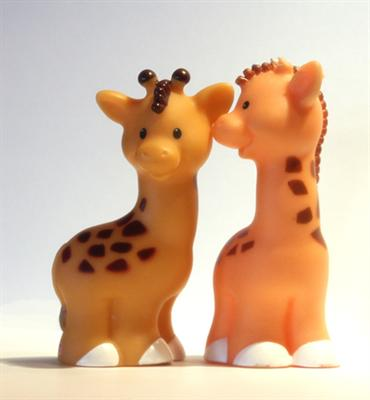
\includegraphics[width=0.6in,height=0.8in]{./Figures/previews/raw.jpg}
    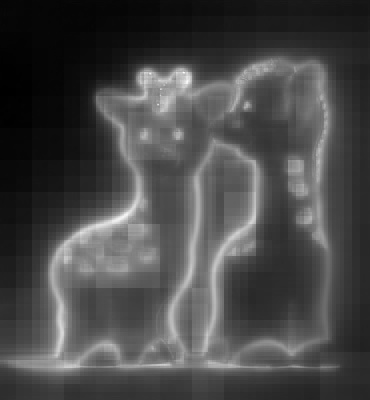
\includegraphics[width=0.6in,height=0.8in]{./Figures/previews/MC.jpg}
    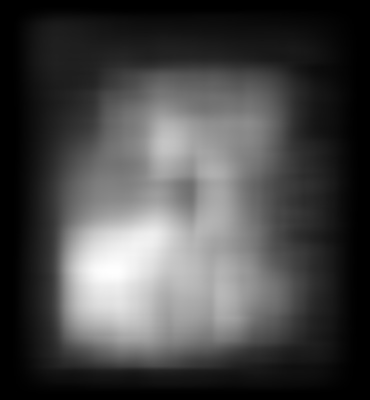
\includegraphics[width=0.6in,height=0.8in]{./Figures/previews/CSH.jpg} 
    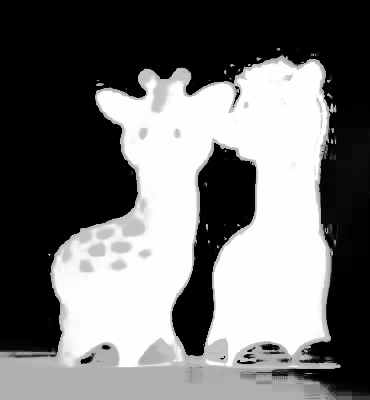
\includegraphics[width=0.6in,height=0.8in]{./Figures/previews/CSD.jpg} 
    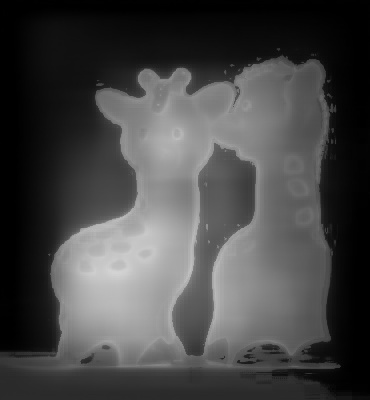
\includegraphics[width=0.6in,height=0.8in]{./Figures/previews/Composed.jpg} \\
    \caption{Original Image and Preview of feature maps}\vspace{1mm}
       \small Left to Right: Original Image, Multiscale Contrast Map, Centre-Surround Histogram, Colour Spatial Distribution, Composed Unary Potentials
\end{center}
\end{figure}

The final value of each feature $F_k(a_x,I)$ comes from a normalised feature map $f_k(x,I)\in[0,1]$, where for each pixel: $$F_k(a_x,I) = \left\{\begin{matrix}f_k(x,I), & a_x=0\\1-f_k(x,I), & a_x=1\end{matrix}\right.$$


%% Feature Extraction (2 pages)
\subsection{Feature Extraction}
Feature Extraction, widely acknowledged as the most significant component of a computer vision task, represents how we want the computer to interpret raw images. In this project, we focus on three features, each of which is capable of capturing saliency individually but in different level of scope. They are respectively multiscale contrast, centre-surround histograms  and colour-spatial distribution. 
%% local feature
\subsubsection{Multiscale Contrast}

Constrast is commonly used as local feature because it simulates the human visual receptive fields. It acts on the fact that the boundary of salient objects tend to have a marked contrast to the surrounding region. Since we may have no prior knowledge about the size of salient object, it is usual to compute the contrast at multiple scales to then incorporate back into one map, since this will demarcate the various boundaries in the image.  This multiscale contrast map is thus a linear combination of image contrast at all levels of an N-level gaussian image pyramid, using the pixels $x$ in the image $I$.  Formally, this amounts to calculating $$f_c(x,I) = \SUM_{n = 1}^{N}\SUM_{x'\in W(x)}||I^n(x)-I^n(x')||^2$$ where W(x) is a window that delineates which area to consider as neighbouring pixels to compare contrast values.

\BOLD{TODO ADD more technical analysis about why we should have multiple scales.}

\begin{figure}[ht]
\begin{center}    
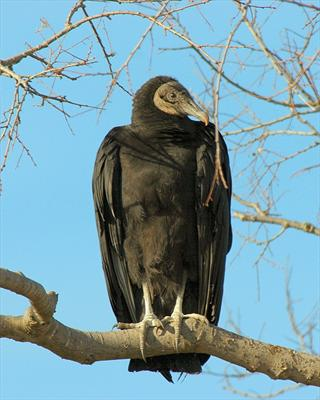
\includegraphics[width=0.65in,height=0.9in]{./Figures/pyramid/5_145_145839raw.jpg} \hspace{2mm}
 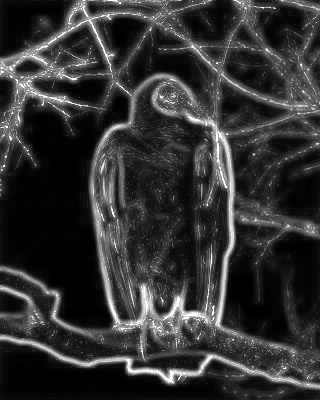
\includegraphics[width=0.65in,height=0.9in]{./Figures/pyramid/5_145_145839_p0.jpg} 
 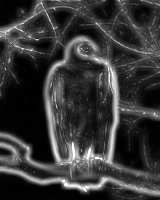
\includegraphics[width=0.325in,height=0.45in]{./Figures/pyramid/5_145_145839_p1.jpg} 
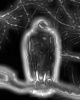
\includegraphics[width=0.1625in,height=0.225in]{./Figures/pyramid/5_145_145839_p2.jpg} 
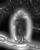
\includegraphics[width=0.08125in,height=0.1125in]{./Figures/pyramid/5_145_145839_p3.jpg} 
 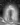
\includegraphics[width=0.040625in,height=0.0575in]{./Figures/pyramid/5_145_145839_p4.jpg} 
 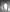
\includegraphics[width=0.0203125in,height=0.02825in]{./Figures/pyramid/5_145_145839_p5.jpg} \hspace{1mm}
 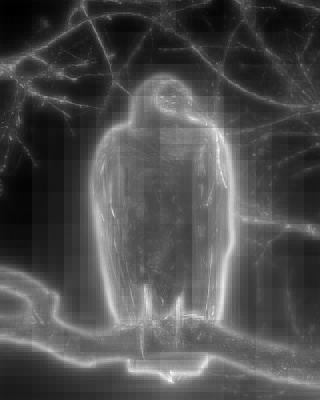
\includegraphics[width=0.65in,height=0.9in]{./Figures/pyramid/5_145_145839.jpg} \\   
\caption{Multiscale Contrast example.}\small{Leftmost: Original Image. Rightmost: Multiscale Feature Map. \\
Immediate images: multiscale pyramids from level $1$ to $6$.}
\end{center}
\end{figure}


In our implementation, we choose the total number of pyramid level $N$ to be $6$ and the size of the window to be $9 \times 9$. 

As can be seen in \BOLD{CONTRAST FIGURE}, the derived multiscale contrast map provides a high distinction between boundary and non-boundary regions. This provides us a precise description of where the boundary of a salient object could exist in the output binary mask. When a salient object also has high contrast inside its boundaries, this feature works perfectl, such as the bird in \BOLD{FIG} and the house in \BOLD{FIG}.

But there are some drawbacks that are tough to avoid. The boundaries of all objects are highlighted, which is not desirable when searching for a single salient object.  This is because we need to give a high probability to marking pixels that are relevant to the salient object rather than every boundary possible. If this doesn't happen, there is the possibility of a "saliency leak" into non-salient areas of the final result that could deteriorate the detector's precision.

\begin{figure}[h]
    \begin{center}
    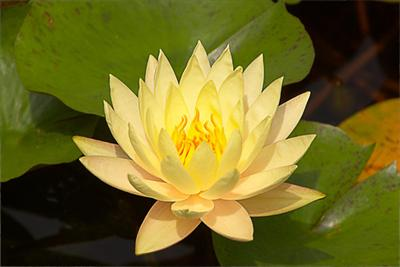
\includegraphics[width=0.7in,height=0.54in]{./Figures/contrast/1orig.jpg}
    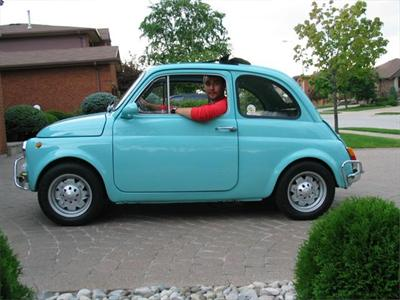
\includegraphics[width=0.7in,height=0.54in]{./Figures/contrast/2orig.jpg}
    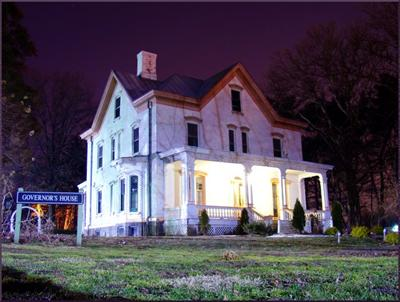
\includegraphics[width=0.7in,height=0.54in]{./Figures/contrast/3orig.jpg}
    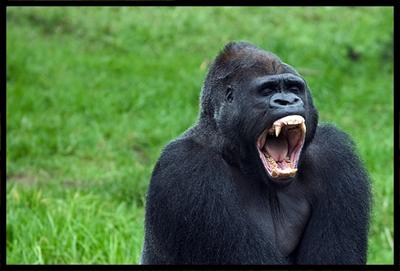
\includegraphics[width=0.7in,height=0.54in]{./Figures/contrast/4orig.jpg}\\
    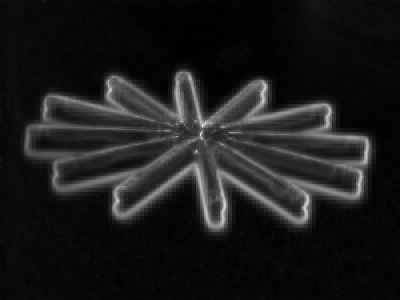
\includegraphics[width=0.7in,height=0.54in]{./Figures/contrast/1cont.jpg}
    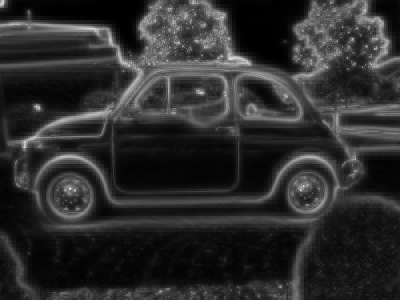
\includegraphics[width=0.7in,height=0.54in]{./Figures/contrast/2cont.jpg}
    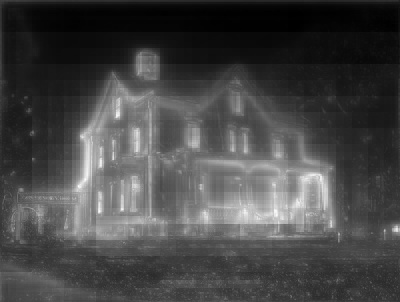
\includegraphics[width=0.7in,height=0.54in]{./Figures/contrast/3cont.jpg}
    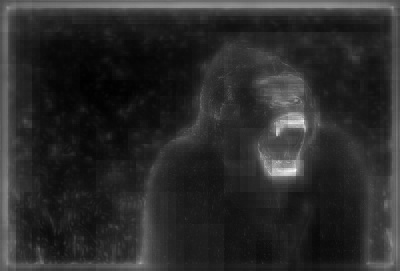
\includegraphics[width=0.7in,height=0.54in]{./Figures/contrast/4cont.jpg}\\
    \footnotesize \hspace{0.1cm} (a) \hs (b) \hs  (c) \hs (d) \\
\caption{Feature Maps of Multiscale Contrast} \label{Fig:LocalFeatureMap}
    \end{center}
\end{figure}

Another disadvantage to only using multiscale contrast is that the inner regions of salient objects are poorly represented.  For example in the gorilla in \BOLD{FIG}, the teeth are labelled as higher contrast to their surroundings compared to that of the body of the gorilla to the grass. Since each entry of the output feature map is quantitatively normalised, the contrast of the gorilla's body to the grass is rendered trivial compared to the contrast of the tooth. The tooth is not what the human receptive field would label as salient because it is a smaller part of the animal, and thus it should not be labelled as the salient object. This flaw may result in low recall comparing to the ground truth data when contrast is used as the sole method to distinguish a salient object.

\subsubsection{Centre-Surround Histogram}
%% regional feature

As shown in \ref{Fig:LocalFeatureMap} , the local feature - multiscale contrast only partially detects salient objects since it is only sensitive to the boundaries. Out of the purpose of detecting the whole block of objects, we make use of another static salient feature, which captures the regional information of saliency and can be computed using various low-level features via a center-surround operation. 

Create a colour RGB histogram for both the rectangle and the surrounding frame, which has the same area with the center rectangle, with a certain resolution (number of ``bins'' for each colour). And then measure the distinguishability of the area centered at each pixel $x$ by calculating the $\chi^2$ value between the two histograms to obtain the differences between the rectangle and the surrounding frame.  Do this for multiple aspect ratios, and keep the largest $\chi^2$ value: 

\begin{align*}
R(x) &= \argmax\limits_{R(x)}\chi^2(R(x), R_s(x)) \\ &=\argmax\limits_{R(x)}\frac{1}{2}\cdot\SUM_{i\in bins}\frac{(hist_{R(x)_i}-hist_{R_s(x)_i})^2}{hist_{R(x)_i}+hist_{R_s(x)_i}}
\end{align*}

Here, we traverse through five template of rectangle with different aspect ratio $\{ 0.5, 0.75, 1.0, 1.25, 1.5\}$ for determining the most distinct pair of centre and surround rectangle centred at each pixel $x$. Besides, to reduce the demands on computational resources, the size range of the rectangle is reduced to 12 discrete ratios $\{$0.18, 0.2, 0.25, 0.3, 0.35, 0.4, 0.45, 0.5, 0.55, 0.6, 0.65, 0.7, 0.75$\}$ with regards to  $min(w,h)$, which is the minimal value of width and height of the processed image.

The centre-surround histogram feature at each pixel $x$ is finally calculated by $$f_h(x,I)\propto\SUM_{x'|x\in R(x')}w_{xx'}\chi^2(R(x'),R_s(x'))$$
Note that the centre-surround histogram feature reflects the distinguishability of each pixel, which is assigned from the distinguishability of the most outstanding area centred at each pixel of one image, with the weight of spatial closeness to the centre of that area. 

\begin{figure}[h]
    \begin{center}
    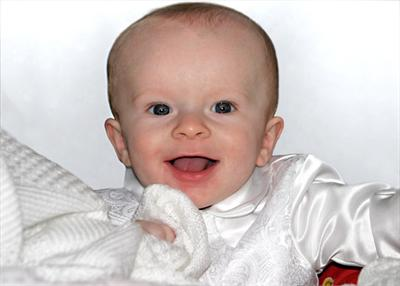
\includegraphics[width=0.7in,height=0.54in]{./Figures/CSH_image/1orig.jpg}
    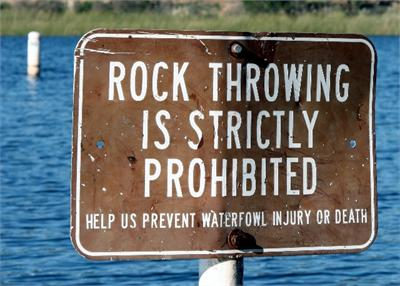
\includegraphics[width=0.7in,height=0.54in]{./Figures/CSH_image/2orig.jpg}
    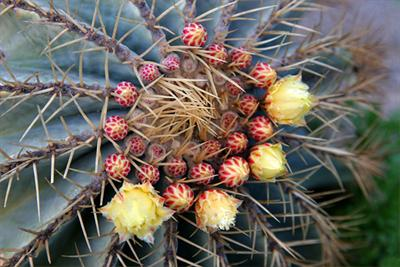
\includegraphics[width=0.7in,height=0.54in]{./Figures/CSH_image/3orig.jpg}
    \includegraphics[width=0.7in,height=0.54in]{./Figures/CSH_image/4orig.jpg}\\
    \includegraphics[width=0.7in,height=0.54in]{./Figures/CSH_image/1cont.jpg}
    \includegraphics[width=0.7in,height=0.54in]{./Figures/CSH_image/2cont.jpg}
    \includegraphics[width=0.7in,height=0.54in]{./Figures/CSH_image/3cont.jpg}
    \includegraphics[width=0.7in,height=0.54in]{./Figures/CSH_image/4cont.jpg}\\
    \footnotesize \hspace{0.1cm} (a) \hs (b) \hs  (c) \hs (d) \\
    \caption{Feature Maps of Centre-Surrond Histograms} \label{Fig:RegionalFeatureMap}
    \end{center}
\end{figure}


As we can see from Fig.\ref{Fig:RegionalFeatureMap}, the whole salient block within one image is
given distinguishable emphasis comparing to its surrounds in the output feature map. 

However, unlike multiscale contrast, the center surround histogram does not provide accurate description for the 
boundary of one object, which is an inherent drawback of this regional feature. Fortunately, 
as mentioned previously, the local feature, to some extent, would complement the regional feature 
at the boundary description. 



%% global feature
\subsubsection{Colour Spatial Distribution}

The goal of using colour spatial distribution feature is to take into account the global 
saliency information, that is, the information about how widely the colours occurring in 
one image are distributed over the global scope. 

First of all, we create the Gaussian Mixture Components $\{c, \mu_c, \Sigma_c\}$ 
with regard to the color component $c$ and fitting these components, making use of pixels of the whole image. 
According to the Gaussian Mixtures Model, each pixel is associated to a colour component with the probability $$
    P(c|I_x) = \frac{\omega_c\mathcal{N}(I_x|\mu_c,\Sigma_c)}{\SUM_c \omega_c \mathcal{N}(I_x|\mu_c,\Sigma_c)}$$ 
where $\omega_c$ is the weight, $\mu_c$ is the mean colour, $\Sigma_c$ is the covariance, and $\mathcal N(I_x|\mu_c,\Sigma_c)$ is the multivariate normal distribution of the $c^{th}$ component. 

For each fitted gaussian colour component $c$, we compute its horizontal variance $V_{h}(c)$ as 
$$V_{h}(c) = \frac{1}{|X|_{c}} \sum_{x} p (c|I_{x}) \cdot | x_{h} - M_{h}(c) |^{2}$$ 
where $x_h$ is horizontal coordinate of pixel $x$, $|X|_c$ is normalising factor and $M_h (c)$ 
is the mean of the gaussian component:
$$|X|_c = \sum_x p(c|I_x)\\M_h (c) = \frac{1}{|X|_c} \sum_{x} p(c|I_x) \cdot x_h$$

Vertical variance $V_{v}(c)$ is defined similarly, and we equally combine the horizontal 
and vertical variance to derive the unnormalised composite variance $V_h (c)$:
$$V' (c) = V_h (c) + V_v (c) $$
Then employ the min-max approach to normalise the composite covariance
$$V (c) = \frac{V'(c) - min \big(V'(c)\big) }{max \big(V'(c)\big) - min \big(V'(c)\big)}$$
where $V(c)$ is the normalised composite covariance of the $c^{th}$ component, contained between 0 and 1.

And then we give penalty to the pixels with high-variance colour, according to the 
supposition that the colour of salient object in one image tends to be intensive in the 
spatial aspect. Thus, the ultimate colour spatial distribution feature for pixel $x$ is defined
as a weighted sum of its color intensiveness $$f_s(x,I)\propto\SUM_c p(c|I_x)\cdot(1-V(c))$$

The feature map $f_s (\cdot,I)$ is also normalized to the range $[0, 1]$. The following figure shows colour spatial distribution feature maps of several example images. The salient objects are well covered by this global feature. 

\begin{figure}[h]
    \begin{center}
    \includegraphics[width=0.72in,height=0.52in]{./CSD_image/1.jpg}
    \includegraphics[width=0.72in,height=0.52in]{./CSD_image/2.jpg}
    \includegraphics[width=0.72in,height=0.52in]{./CSD_image/3.jpg}
    \includegraphics[width=0.72in,height=0.52in]{./CSD_image/4.jpg}\\
    \includegraphics[width=0.72in,height=0.52in]{./CSD_image/1_CSD.jpg}
    \includegraphics[width=0.72in,height=0.52in]{./CSD_image/2_CSD.jpg}
    \includegraphics[width=0.72in,height=0.52in]{./CSD_image/3_CSD.jpg} 
    \includegraphics[width=0.72in,height=0.52in]{./CSD_image/4_CSD.jpg} \\
    \footnotesize \hspace{0.1cm} (a) \hs (b) \hs  (c) \hs (d) \\
     \caption{Feature Maps of Color Spatial Distribution} \label{Fig:GlobalFeatureMap}
    \end{center}
\end{figure}

It is evident that the global feature gains a huge success in mark up the saliency when the background is monotonous. As illustrated by the first three images in the above figure, the flying stuff is distinguished from the bichrome background - blue ocean and white tide, the sign card under the  background of ocean and tree leaves and in the third image the girl body before the fully white wall.

However, in the case of colorful background, color spatial distribution, with a high probability, fails to distinguish the salient object in the image. The Fig.\ref{Fig:GlobalFeatureMap} (d) demonstrates us this undesired property of the global feature. 

One variation in our implementation is to create the component model from only a subset of the pixels in the image. The pixels in the subset is picked up with equal spatial distance. Specifically, we apply the "pydown" module in Opencv to dilute the pixels participating this unsupervised learning task. Such manipulation will not sacrifice too much accuracy, but greatly reduce  the running time of fitting the Mixture of Gaussians since the number of pixels provided for the fitting halves. 

\begin{figure}[h]
    \begin{center}
    \includegraphics[width=0.72in,height=0.52in]{./Figures/pydownCompare/1.jpg}
    \includegraphics[width=0.72in,height=0.52in]{./Figures/pydownCompare/1NOPYDOWN.jpg}
    \includegraphics[width=0.72in,height=0.52in]{./Figures/pydownCompare/1PYDOWN.jpg} 
    \includegraphics[width=0.72in,height=0.52in]{./Figures/pydownCompare/1DOUBLEPYDOWN.jpg} \\
    \includegraphics[width=0.72in,height=0.52in]{./Figures/pydownCompare/2.jpg}
    \includegraphics[width=0.72in,height=0.52in]{./Figures/pydownCompare/2NOPYDOWN.jpg}
    \includegraphics[width=0.72in,height=0.52in]{./Figures/pydownCompare/2PYDOWN.jpg} 
    \includegraphics[width=0.72in,height=0.52in]{./Figures/pydownCompare/2DOUBLEPYDOWN.jpg} \\
    \includegraphics[width=0.72in,height=0.52in]{./Figures/pydownCompare/3.jpg}
    \includegraphics[width=0.72in,height=0.52in]{./Figures/pydownCompare/3NOPYDOWN.jpg}
    \includegraphics[width=0.72in,height=0.52in]{./Figures/pydownCompare/3PYDOWN.jpg} 
    \includegraphics[width=0.72in,height=0.52in]{./Figures/pydownCompare/3DOUBLEPYDOWN.jpg} \\
    \footnotesize (a) original (b) no pydown (c) one-level pydown (d) two-level pydown
    \caption{Examples for global feature using diluted images} \label{Fig:GlobalPydown}
    \end{center}
\end{figure}

We test three levels of pixel dilution: no pydown, one-level pydown and two-level pydown. 
One-level pydown means reducing both of the width and height of one image to half of the 
original size,  such that only a quarter of pixels are available for fitting the mixture 
of gaussians. From the above figure, it is evident that one-level pydown, to some extent, 
increases the quality of  this global feature by marking the salient block softly or 
obscurely rather than in a strict way. 

Extraction for two-level pydown indicated in Fig.\ref{Fig:GlobalPydown} (d) is even faster, but generally 
it lost the effectiveness of this global feature.

Hence, in our implementation of color spatial distribution, we employ the one-level 
pydown as a trick to both enhance quality of global feature and improve extraction time performance.

Besides, the maximum number of iterations is limited $(100)$ and the convergence criterion 
is lowered $(10^{-1})$ in order to reduce the time taken to compute this feature.  This 
outcome of this global feature, after such simplification, will not get deteriorated 
since we only care about capturing  approximate component location, rather than precisely
maximum likelihood of the coloured pixels.

The number of gaussian components is another trade-off between the quality of 
feature extraction and computational cost. Our implementation uses five gaussians 
to softly capture color components in one image. 


%% Learning (0.5 page)
\subsection{Learning}
Those three features aforementioned have their own strengthes and weaknesses in 
different areas. For example, the \BOLD{CONTINUE}

It goes without saying that incorporating all three features into the unary potential of the CRF model to complement each other. It would be oversimplistic and unpersuasive to treat three features in equal weight since one feature perhaps may be stronger than other two features and ought to be assigned with higher importance. Hence, one effective and reasonable approach is to adjustably determine the optimal weight to combine three features with the help of certain machine learning algorithm. 

In this project, we implement logistic regression to decide the optimal weight under the help of training data.

%% CRF Inference (0.5 - 1 page)
%% images for inferred binary mask
\subsection{CRF Inference}
To infer the maximum likelihood assignment for pixelwise variables under the CRF framework, the usual message passing algorithm would be intractable. Therefore, we turn to the $\alpha$-expansion inference,
which successively segments all and non-$\alpha$ pixels with graph cuts and the algorithm will change the value of $\alpha$ at each iteration with graph-cut algorithm. By this means, inferring maximum likelihood assignment for binary saliency variable, or equivalently, 
 minimal energy function would be much faster. 

But how to determine the parameter $\lambda_0$, which indicates to what extent, relative to the unary term (combined feature map), we ought to consider the pairwise potential in deciding the binary saliency of one pixel? And this parameter would influence the smoothness of resulting binary mask since pairwise term can be regarded as the penalty to adjacent pixels with different labels. Our solution is to determine the optimal $\lambda_0$ by applying the cross validation on $\lambda_0$ at various magnitudes. 

\BOLD{TODO add diagram and graph to illustrate our cross validation on various lambda
TODO:add diagram and graph to illustrate our cross validation on various lambda}

By cross validation above, the optimal parameter $\lambda_0$ we use for evaluating the binary mask is $\lambda_0 = 8$.

\begin{figure}[h]
\begin{center}
    \includegraphics[width=0.8in,height=0.6in]{./Figures/CRFinference/5_159_159364.jpg}
    \includegraphics[width=0.8in,height=0.6in]{./Figures/CRFinference/5_159_159364_3.jpg}
    \includegraphics[width=0.8in,height=0.6in]{./Figures/CRFinference/5_159_159364_2.jpg} \\
    \includegraphics[width=0.8in,height=0.6in]{./Figures/CRFinference/5_159_159649.jpg}
    \includegraphics[width=0.8in,height=0.6in]{./Figures/CRFinference/5_159_159649_3.jpg}
    \includegraphics[width=0.8in,height=0.6in]{./Figures/CRFinference/5_159_159649_2.jpg} \\
    \includegraphics[width=0.8in,height=0.6in]{./Figures/CRFinference/5_162_162349.jpg}
    \includegraphics[width=0.8in,height=0.6in]{./Figures/CRFinference/5_162_162349_3.jpg}
    \includegraphics[width=0.8in,height=0.6in]{./Figures/CRFinference/5_162_162349_2.jpg} \\
    \footnotesize  (a) Raw Image (b) Combined Unary Map  (c) Binary Mask ($\lambda=8$)\\
     \caption{Examples for CRF inference by $\alpha$-algorithm}
\end{center}
\end{figure}

%% Result evaluation in rectangle level (1 page)
%% images for the output rectangle
\section{Result Evaluation}
We randomly pick up 1000 images from MSRA dataset B to form the training set.
And we choose another 500 images to form the testing set.

\subsection{Bounding Box}
The binary mask derived from the CRF inference can be used directly in a multitude of applications. However, in order to evaluate the accuracy of our approach, we make use of OpenCV's findContours algorithm to output a bounding box around the salient object, based on the derived pixel-wise binary mask. The dimensions of this bounding box is output as a label for each image into a text file holding all resultant labels for that directory.

%% TODO Specific algorithm for output bounding box

\begin{figure}[h]
\begin{center}
    \includegraphics[width=0.6in,height=0.4in]{./Figures/boundingbox/5_145_145114RECT.jpg}
    \includegraphics[width=0.6in,height=0.4in]{./Figures/boundingbox/5_145_145275RECT.jpg}
    \includegraphics[width=0.6in,height=0.4in]{./Figures/boundingbox/5_145_145349RECT.jpg}
    \includegraphics[width=0.6in,height=0.4in]{./Figures/boundingbox/5_145_145398RECT.jpg}
    \includegraphics[width=0.6in,height=0.4in]{./Figures/boundingbox/5_146_146319RECT.jpg} \\
    \includegraphics[width=0.6in,height=0.4in]{./Figures/boundingbox/5_146_146330RECT.jpg}
    \includegraphics[width=0.6in,height=0.4in]{./Figures/boundingbox/5_146_146332RECT.jpg}
    \includegraphics[width=0.6in,height=0.4in]{./Figures/boundingbox/5_146_146431RECT.jpg}
    \includegraphics[width=0.6in,height=0.4in]{./Figures/boundingbox/5_146_146552RECT.jpg}
    \includegraphics[width=0.6in,height=0.4in]{./Figures/boundingbox/5_147_147367RECT.jpg} \\
    \includegraphics[width=0.6in,height=0.4in]{./Figures/boundingbox/5_148_148067RECT.jpg}
    \includegraphics[width=0.6in,height=0.4in]{./Figures/boundingbox/5_148_148271RECT.jpg}
    \includegraphics[width=0.6in,height=0.4in]{./Figures/boundingbox/5_148_148710RECT.jpg}
    \includegraphics[width=0.6in,height=0.4in]{./Figures/boundingbox/5_148_148763RECT.jpg}
    \includegraphics[width=0.6in,height=0.4in]{./Figures/boundingbox/5_148_148788RECT.jpg} \\
    \includegraphics[width=0.6in,height=0.4in]{./Figures/boundingbox/5_150_150590RECT.jpg}
    \includegraphics[width=0.6in,height=0.4in]{./Figures/boundingbox/5_151_151334RECT.jpg}
    \includegraphics[width=0.6in,height=0.4in]{./Figures/boundingbox/5_153_153455RECT.jpg}
    \includegraphics[width=0.6in,height=0.4in]{./Figures/boundingbox/5_153_153651RECT.jpg}
    \includegraphics[width=0.6in,height=0.4in]{./Figures/boundingbox/5_154_154297RECT.jpg} \\
    \includegraphics[width=0.6in,height=0.4in]{./Figures/boundingbox/5_155_155096RECT.jpg}
    \includegraphics[width=0.6in,height=0.4in]{./Figures/boundingbox/5_155_155145RECT.jpg}
    \includegraphics[width=0.6in,height=0.4in]{./Figures/boundingbox/5_155_155333RECT.jpg}
    \includegraphics[width=0.6in,height=0.4in]{./Figures/boundingbox/5_155_155196RECT.jpg}
    \includegraphics[width=0.6in,height=0.4in]{./Figures/boundingbox/5_155_155459RECT.jpg} \\
    \caption{Examples images for bounding box output}
\end{center}
\end{figure}

% TODO add some analysis here.

\subsection{Evaluation Criteria}
%% why we need evaluation criteria
The main functionality of evaluation criteria is to measure the effectiveness of our approach.
In our project, evaluation will be applied, as well, in the cross validation while determining the 
energy function parameter $\lambda_0$. 
But what kind of criteria could effectively capture the goodness of our model?
As to this project, we utilise the both the region-based and boundary-based measurements proposed by Tie. Liu.

\subsubsection{Region-based measurement}
Precision and Recall, both taking significant roles in the information retrival as performance indicator,
are utilised in this project to evaluate the correctness of our output rectangle. 

The precision represents the percentage of pixels that are correctly detected in ground truth, which 
is the ratio of the number of pixels in overlapped region to pixel number contained in the ground truth box.
And the recall reflects the percentage of pixels that are correctly detected in resulted detection, 
which is the ratio of pixel number the overllapped region contained to the number of pixels.
%% explain what is by graph and diagram

\begin{figure}[h]
\begin{center}
    \includegraphics[width=1.0in,height=0.8in]{Figures/Creteria/B.jpg}
    \includegraphics[width=1.0in,height=0.8in]{Figures/Creteria/C.jpg} 
    \includegraphics[width=1.0in,height=0.8in]{Figures/Creteria/A.jpg} \\
    \footnotesize (a) \hs \hspace*{0.8cm} (b)  \hs \hspace*{0.8cm} (c)
    \caption{Examples with resulted detection and ground truth} \label{Fig:PrecisionANDRecall}
    \footnotesize Red Box: ground truth label. Green Box: resulted detection
\end{center} \end{figure}

It is evident that all threes detections in Fig.\ref{Fig:PrecisionANDRecall} is far from satisfying. 
The salient detection in the leftmost image, the precision is 100\% while the recall is small.
Such detection is not desired because of the failure to detect all pixels within the true salient object.
On top of that, the detection in the middle image has 100\% recall, however, 
the precision is low in that a large portion of non-salient pixels are returned as the detection result.

For an overall performance measurement, we use the F-measure indicator with $\alpha = 0.5$, which is the weighted 
harmonic mean of precision and recall:
$$
    F_{0.5} = \frac{1.5\times Precision \times Recall}{ 0.5 \times Precision + Recall}
$$

\subsubsection{Boundary-based measurement}
The Boundary Displacement Error (BDE) measures the average of positional difference 
of ground truth and resulted detection. \\
\BOLD{Add brief math description of BDE here?}

%% Discussion (existing flaws and possible improvements) (0.5 page)
\section{Conclusion and Discussion}
In this project, we have indicated a supervised approach for salient object detection 
which is formulated as a binary labeling problem using a set of local, regional,
and global salient object features.

%% flaws in our project
However, out of the limitation of time, one flaw of our project is the lack of comparison
with other approaches using the numerical evaluation result, which may tremendously 
enhance the persuasiveness of the approache utlised in this project. 

\BOLD{Multiple object detection?}

%% technical enhancement?
There are still several remaining issues for further investigation. 
\BOLD{multiple }

%% acknowlegement and reference (0.5 page)
\begin{thebibliography}{99} \fontsize{9pt}{50} \setlength{\itemsep}{-0.5pt} 
    \bibitem 1 Liu, Tie, et al. "Learning to detect a salient object." 
        \textit{Computer Vision and Pattern Recognition, 2007. CVPR07. IEEE Conference on. IEEE, 2007}.

    \bibitem 2 Liu, Tie, et al. "Learning to detect a salient object." 
        \textit{Pattern Analysis and Machine Intelligence, IEEE Transactions on 33.2 (2011): 353-367}. 

    \bibitem 3 Itti, Laurent, Christof Koch, and Ernst Niebur. "A model of saliency-based visual attention for rapid scene analysis."
        \textit{Pattern Analysis and Machine Intelligence, IEEE Transactions on 20.11 (1998): 1254-1259}.

    \bibitem 4 Ma, Yu-Fei, and Hong-Jiang Zhang. "Contrast-based image attention analysis by using fuzzy growing."
        \textit{ Proceedings of the eleventh ACM international conference on Multimedia. ACM, 2003}. 

    \bibitem 5 L. Itti. Models of Bottom-Up and Top-Down Visual Attention. PhD thesis, 
        \textit{California Institute of Technology Pasadena, 2000}.

    \bibitem 6 Boykov, Yuri, Olga Veksler, and Ramin Zabih. "Fast approximate energy minimization via graph cuts." 
        \textit{Pattern Analysis and Machine Intelligence, IEEE Transactions on 23.11 (2001): 1222-1239}.

    \bibitem 7 Suzuki, S. and Abe, K., Topological Structural Analysis of Digitized Binary Images by Border Following. 
        \textit{CVGIP 30 1, pp 32-46 (1985)}.

    \bibitem 8 Gould, Stephen. "DARWIN: A Framework for Machine Learning and Computer Vision Research and Development." 
        \textit{Journal of Machine Learning Research 13 (2012): 3533-3537}.

\end{thebibliography}
%-------------------------------------------------------------------------

\end{document}
